%!TeX program = xelatex
\PassOptionsToPackage{most}{tcolorbox}
\documentclass[12pt,a4paper,UTF8]{ctexart}
\usepackage{UCASReport}
\usepackage{placeins}

\newcommand{\unnumberedsection}[1]{%
  \refstepcounter{section}%
  \setcounter{subsection}{0}%
  \section*{#1}%
}
\newcommand{\testphoto}[3]{%
    \begin{minipage}{0.48\textwidth}
        \centering
        \IfFileExists{#1}{%
            \includegraphics[width=\linewidth]{#1}%
        }{%
            \fbox{\parbox[c][0.22\textwidth][c]{0.92\linewidth}{\centering #3}}%
        }%
        \caption{#2}
    \end{minipage}%
}

\setlength{\headheight}{15pt}
\emergencystretch=2em

%%-------------------------------正文开始---------------------------%%
\begin{document}

%%------------------------正文页从这里开始-------------------%
\newpage
\setcounter{page}{1} % 重置页码为1

%%------------------------正文内容从这里开始-------------------%
\section{十进制数字钟}

\subsection{实验原理}

本实验的任务是在 FPGA 开发板上实现一个十进制数字钟，显示格式为 HH:MM:SS。整个系统以开发板提供的 100 MHz 时钟为统一时序基准，在此基础上分出计时用的 1 Hz 脉冲和数码管扫描用的 1 kHz 脉冲。系统总体结构如图 \ref{fig:system_structure} 所示，可以分为时钟分频、时间计数、按键调时、闹钟控制、整点报时和数码管动态显示几个部分。复位信号同时送到各个时序模块，用于把计数器、显示选择和报警状态恢复到初始状态。

\begin{figure}[!htbp]
    \centering
    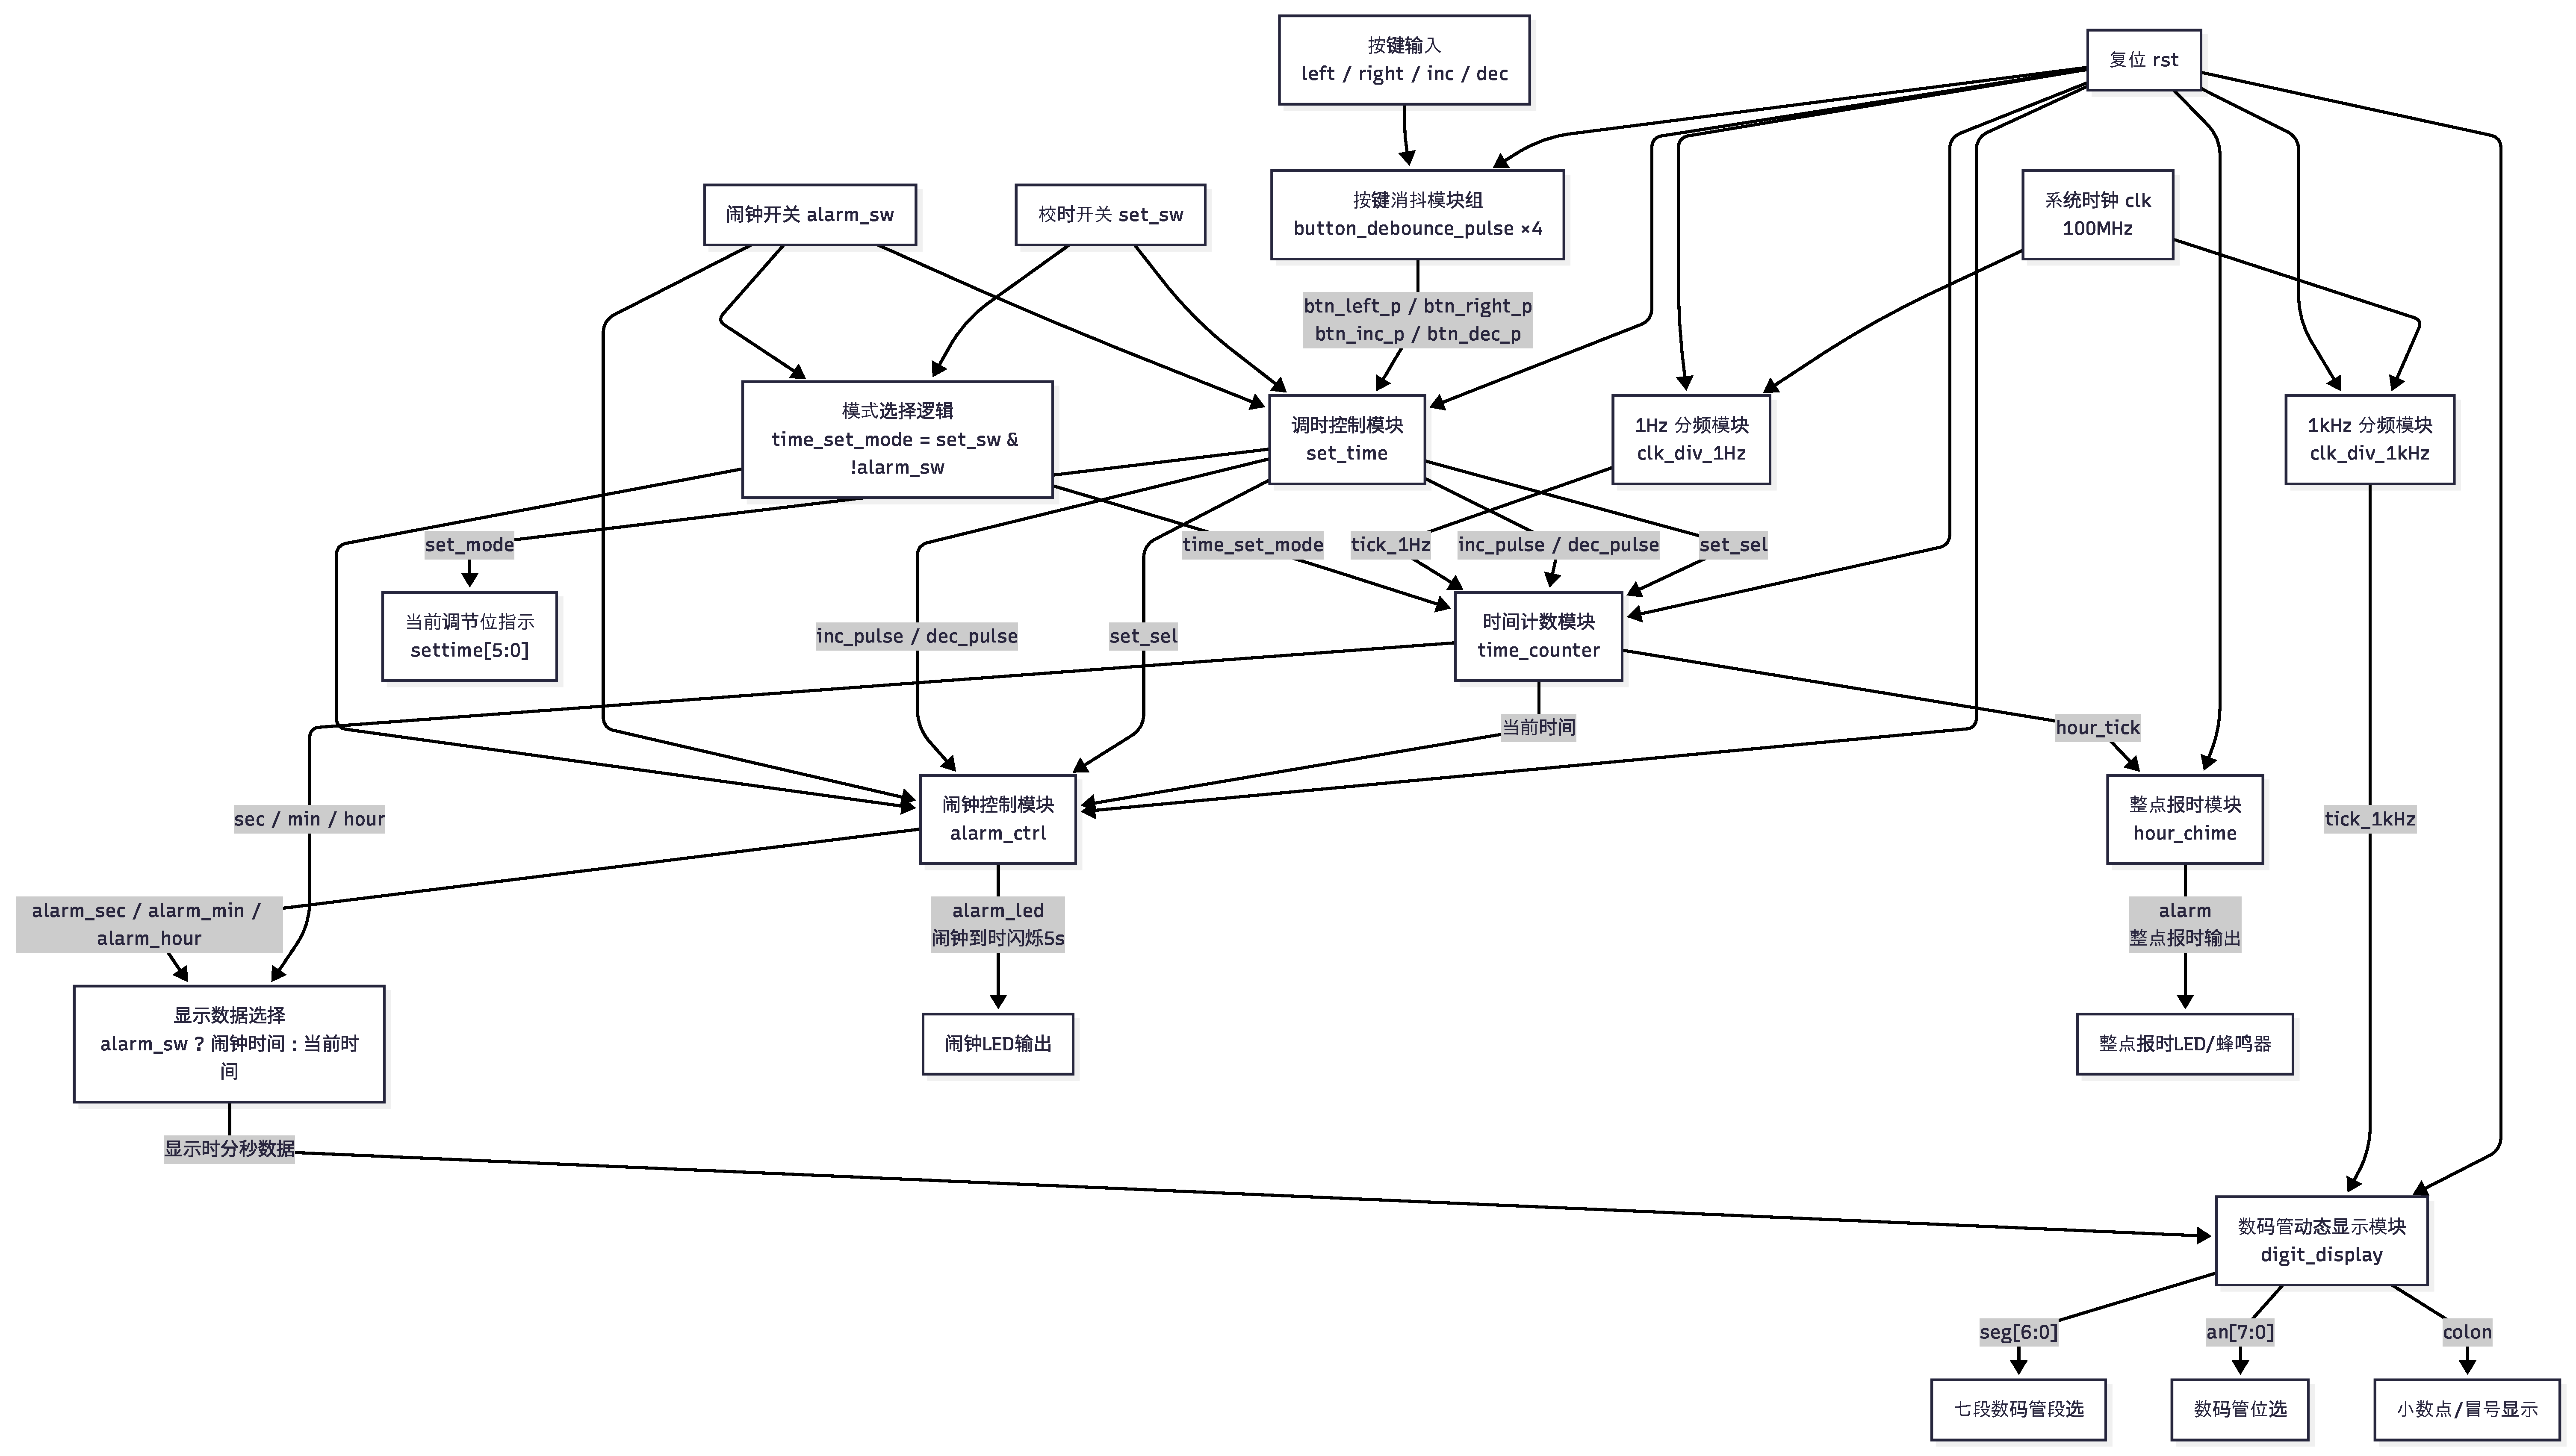
\includegraphics[width=0.98\textwidth]{figures/系统总体结构框图.pdf}
    \caption{数字钟系统总体结构框图}
    \label{fig:system_structure}
\end{figure}

从图 \ref{fig:system_structure} 可以看出，分频模块是整个数字钟的基础。由于 100 MHz 时钟远高于数字钟实际需要的计时速度，所以需要通过计数分频得到较低频率的使能信号。其中 \texttt{tick\_1Hz} 用于驱动秒计数，每产生一次脉冲，时间计数模块更新一次；\texttt{tick\_1kHz} 用于数码管动态扫描，使多个数码管轮流点亮并形成稳定显示。

时间计数模块可以看作多个十进制计数器的级联，其核心状态转移关系如图 \ref{fig:counter_state} 所示。系统复位后显示 00:00:00，并进入等待 1 Hz 脉冲的状态。当 \texttt{tick\_1Hz} 到来时，秒个位先加一；如果秒个位没有达到 9，则只更新秒个位；如果秒个位等于 9，则秒个位清零并向秒十位进位。秒十位、分钟个位和分钟十位也采用类似的进位方式。小时部分使用 24 小时制，因此不能只按普通十进制进位处理，而是需要判断当前小时是否已经到达 23。当时间为 23:59:59 时，再来一个计时脉冲后系统回到 00:00:00。

\begin{figure}[!htbp]
    \centering
    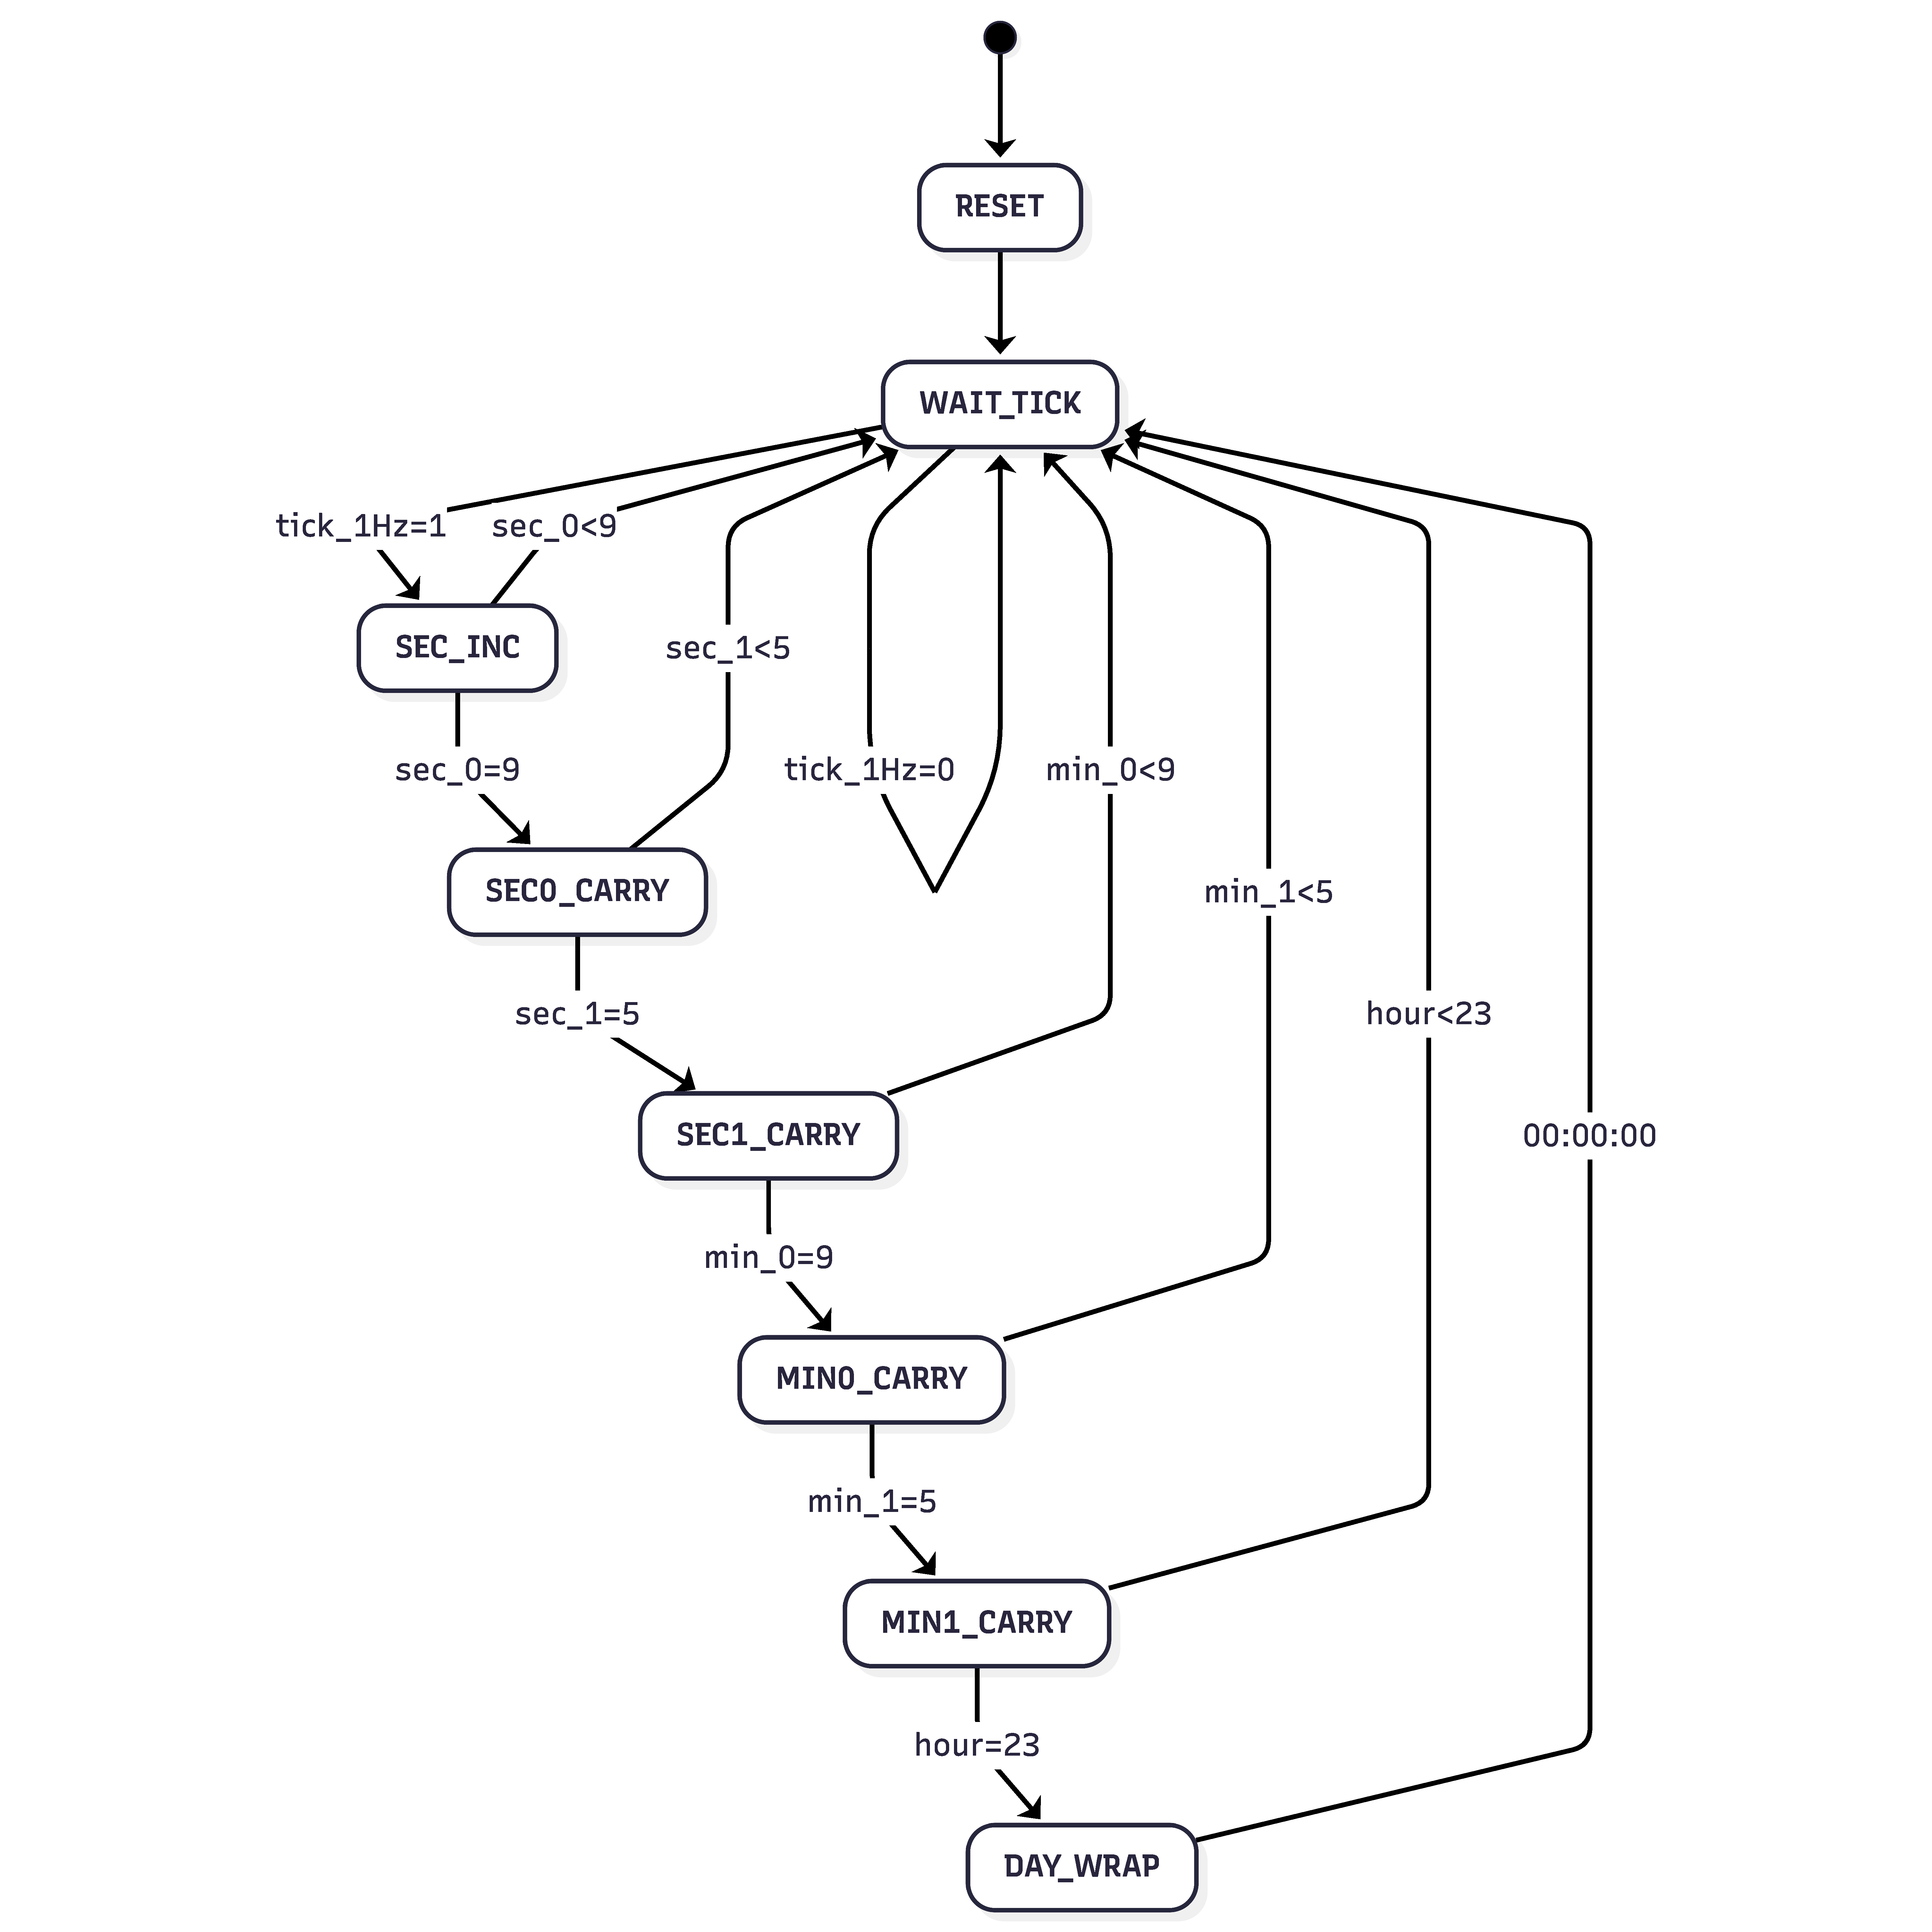
\includegraphics[width=0.60\textwidth]{figures/计时核心逻辑状态图.pdf}
    \caption{计时核心逻辑状态图}
    \label{fig:counter_state}
\end{figure}

显示部分采用数码管动态扫描方式。六位时间数据先由显示数据选择逻辑确定来源：正常情况下显示当前时间，打开闹钟设置开关时显示闹钟时间。随后显示模块在 1 kHz 扫描脉冲控制下依次选通小时十位、小时个位、分钟十位、分钟个位、秒十位和秒个位，并把对应的 BCD 数字译码成七段码。虽然同一时刻实际上只有一位数码管被点亮，但由于扫描速度较快，人眼会看到六位数码管同时显示。

为了实现手动校时，系统设置了校时模式。进入校时模式后，普通的 1 Hz 自动计时暂时停止，左右按键用于选择当前被修改的时间位，加一和减一按键用于改变该位数值。由于机械按键在按下和松开时会产生抖动，如果直接接入计数逻辑，可能一次按键被识别成多次，所以按键信号需要先经过同步、消抖和单脉冲处理，再送入调时控制模块。

在基本数字钟功能之外，本设计还加入了整点报时和闹钟功能。整点报时模块由小时进位信号触发，当时间从 xx:59:59 进入下一小时时输出短暂提示信号。闹钟模块保存一组独立的闹钟时间，在正常计时状态下持续比较当前时间和闹钟时间；当时、分、秒六位数字完全相同时，输出报警信号并让 LED 闪烁一段时间。这样，计时、显示、调时和报警功能之间既通过信号连接形成整体，又保持了比较清楚的模块边界。

\subsection{程序代码}

完整 Verilog 源代码见：\url{https://github.com/AncauqL/Digital_Lab_03}。限于篇幅，报告中只呈现比较关键的代码片段。

\subsubsection{分频模块}

分频模块的思想是用一个计数器数系统时钟周期。开发板时钟是 100 MHz，也就是一秒钟有 $100\,000\,000$ 个时钟周期，所以计数器从 0 数到 $99\,999\,999$ 时，就说明一秒到了。

\begin{codeblock}{Verilog}
reg [26:0] count; // 100M 需要 27 位计数器才能装下

always @(posedge clk) begin
    if (rst) begin
        count <= 0;       // 复位时计数器清零
        tick_1Hz <= 0;   
    end else begin
        if (count == 27'd99_999_999) begin
            count <= 0;       // 数够一秒后重新开始数
            tick_1Hz <= 1;    // 只输出一个时钟周期的高电平
        end else begin
            count <= count + 1;
            tick_1Hz <= 0;    // 还没到一秒时保持为 0
        end
    end
end
\end{codeblock}

1 kHz 分频的写法和上面类似，只是计数终值改成 $99\,999$，这样每 $100\,000$ 个系统时钟周期产生一次扫描脉冲。

\subsubsection{时分秒计数模块}

秒和分钟都可以拆成个位和十位来处理。为了减少重复代码，我写了一个可以设置最大值的通用计数器。秒个位、分个位的最大值是 9；秒十位、分十位的最大值是 5。下面代码里先判断复位，然后判断校时按键，最后才判断正常计时使能。

\begin{codeblock}{Verilog}
assign carry = en && (q == MAX);
// q 到最大值时，如果 en 有效，就给后一位一个进位信号

always @(posedge clk) begin
    if (rst) begin
        q <= 4'd0; // 复位后本位数字变成 0
    end else if (edit_en && inc_pulse) begin
        // 校时模式下按加一键
        if (q == MAX)
            q <= 4'd0; // 加到最大值后再加就回到 0
        else
            q <= q + 1'b1;
    end else if (edit_en && dec_pulse) begin
        // 校时模式下按减一键
        if (q == 4'd0)
            q <= MAX; // 从 0 再减就回到最大值
        else
            q <= q - 1'b1;
    end else if (en) begin
        // 普通计时时，由前一位进位或者 1Hz tick 触发
        if (q == MAX)
            q <= 4'd0;
        else
            q <= q + 1'b1;
    end
end
\end{codeblock}

小时部分单独写，是因为小时最大只能到 23。例如当前是 19，调小时十位时如果变成 29 就是不合法的，所以代码中需要把小时个位修正到 3 以下。正常计时时，当小时为 23 且分钟秒钟也进位时，小时回到 00。

\subsubsection{数码管动态扫描模块}

数码管显示的关键是“扫描”。这里用 \texttt{scan} 表示当前正在显示第几位。每来一次 1 kHz 扫描脉冲，\texttt{scan} 加一，从 0 到 5 循环。不同的 \texttt{scan} 值对应不同的位选信号和不同的时间数字。

\begin{codeblock}{Verilog}
always @(posedge clk) begin
    if (rst) begin
        scan <= 3'd0; // 从第一位开始扫
    end else if (tick_1kHz) begin
        if (scan == 3'd5)
            scan <= 3'd0; // 六位都扫完后回到第一位
        else
            scan <= scan + 1'b1;
    end
end

always @(*) begin
    an = 8'b11111111; // 先默认所有数码管都不亮
    colon = 1'b1;
    current_num = 4'd0;

    case (scan)
        3'd0: begin
            an = 8'b01111111; // 小时十位
            current_num = hour_1;
        end
        3'd1: begin
            an = 8'b10111111; // 小时个位
            current_num = hour_0;
            colon = 1'b0;     // 用小数点当分隔符
        end
        3'd2: begin
            an = 8'b11011111; // 分钟十位
            current_num = min_1;
        end
        3'd3: begin
            an = 8'b11101111; // 分钟个位
            current_num = min_0;
            colon = 1'b0;
        end
        3'd4: begin
            an = 8'b11110111; // 秒十位
            current_num = sec_1;
        end
        3'd5: begin
            an = 8'b11111011; // 秒个位
            current_num = sec_0;
        end
    endcase
end
\end{codeblock}

\subsubsection{校时与按键处理模块}

校时模块主要维护一个 \texttt{set\_sel}，表示现在选中哪一位。这里规定 0-5 分别表示秒个位、秒十位、分钟个位、分钟十位、小时个位和小时十位。按右键时选中位加一，按左键时选中位减一，超过范围后循环回来。

\begin{codeblock}{Verilog}
assign set_mode = set_sw;
assign inc_pulse = set_mode && btn_inc_pulse;
assign dec_pulse = set_mode && btn_dec_pulse;

always @(posedge clk) begin
    if (rst) begin
        set_sel <= 3'd0; // 默认选中秒个位
    end else if (!set_mode) begin
        set_sel <= 3'd0; // 退出校时后也回到默认位置
    end else begin
        if (btn_right_pulse) begin
            if (set_sel == 3'd5)
                set_sel <= 3'd0; // 最左边再右移就回到最右边
            else
                set_sel <= set_sel + 1'b1;
        end else if (btn_left_pulse) begin
            if (set_sel == 3'd0)
                set_sel <= 3'd5; // 最右边再左移就回到最左边
            else
                set_sel <= set_sel - 1'b1;
        end
    end
end
\end{codeblock}

按键消抖模块先用两个寄存器把外部按键同步到系统时钟域，再用计数器判断按键状态是否保持稳定。如果状态稳定时间足够长，就更新按键状态，并且只在按下的那个瞬间输出一个脉冲。

\begin{codeblock}{Verilog}
always @(posedge clk) begin
    if (rst) begin
        btn_meta <= 1'b0;
        btn_sync <= 1'b0;
        btn_state <= 1'b0;
        cnt <= 21'd0;
        pulse <= 1'b0;
    end else begin
        btn_meta <= btn;       // 第一级同步
        btn_sync <= btn_meta;  // 第二级同步
        pulse <= 1'b0;         // 默认不输出脉冲

        if (btn_sync == btn_state) begin
            cnt <= 21'd0; // 状态没变，不需要继续计数
        end else begin
            if (cnt == CNT_MAX) begin
                btn_state <= btn_sync; // 状态稳定后才真正更新
                cnt <= 21'd0;
                if (btn_sync == 1'b1)
                    pulse <= 1'b1; // 只在按下时输出一个脉冲
            end else begin
                cnt <= cnt + 1'b1;
            end
        end
    end
end
\end{codeblock}

\subsubsection{闹钟与整点报时模块}

闹钟模块的基本思路是保存一个闹钟时间，然后在正常计时状态下和当前时间做比较。只有闹钟已经设置有效、没有处在闹钟设置模式、也没有处在普通校时模式时，才允许触发闹钟。

\begin{codeblock}{Verilog}
wire alarm_match =
    alarm_valid &&          // 已经设置过闹钟
    !alarm_sw &&            // 现在不在闹钟设置界面
    !time_set_mode &&       // 现在也不在普通校时界面
    cur_sec_0  == alarm_sec_0  &&
    cur_sec_1  == alarm_sec_1  &&
    cur_min_0  == alarm_min_0  &&
    cur_min_1  == alarm_min_1  &&
    cur_hour_0 == alarm_hour_0 &&
    cur_hour_1 == alarm_hour_1;
\end{codeblock}

当闹钟匹配到目标时间后，系统进入响铃状态。这里没有真正接蜂鸣器，而是用 LED 闪烁表示闹钟触发。整点报时的原理类似，只不过触发条件不是和闹钟时间比较，而是检测分钟向小时进位。

\subsection{仿真结果及分析}

由于顶层模块中 1 Hz 分频器需要计满 $100\,000\,000$ 个系统时钟周期，如果直接仿真完整顶层，等待时间较长，所以仿真时选取关键功能模块进行验证。主要仿真内容包括计时进位、数码管动态扫描、校时与按键消抖、闹钟触发四部分，仿真结果如图所示。

\begin{figure}[htbp]
    \centering
    \begin{minipage}{0.48\textwidth}
        \centering
        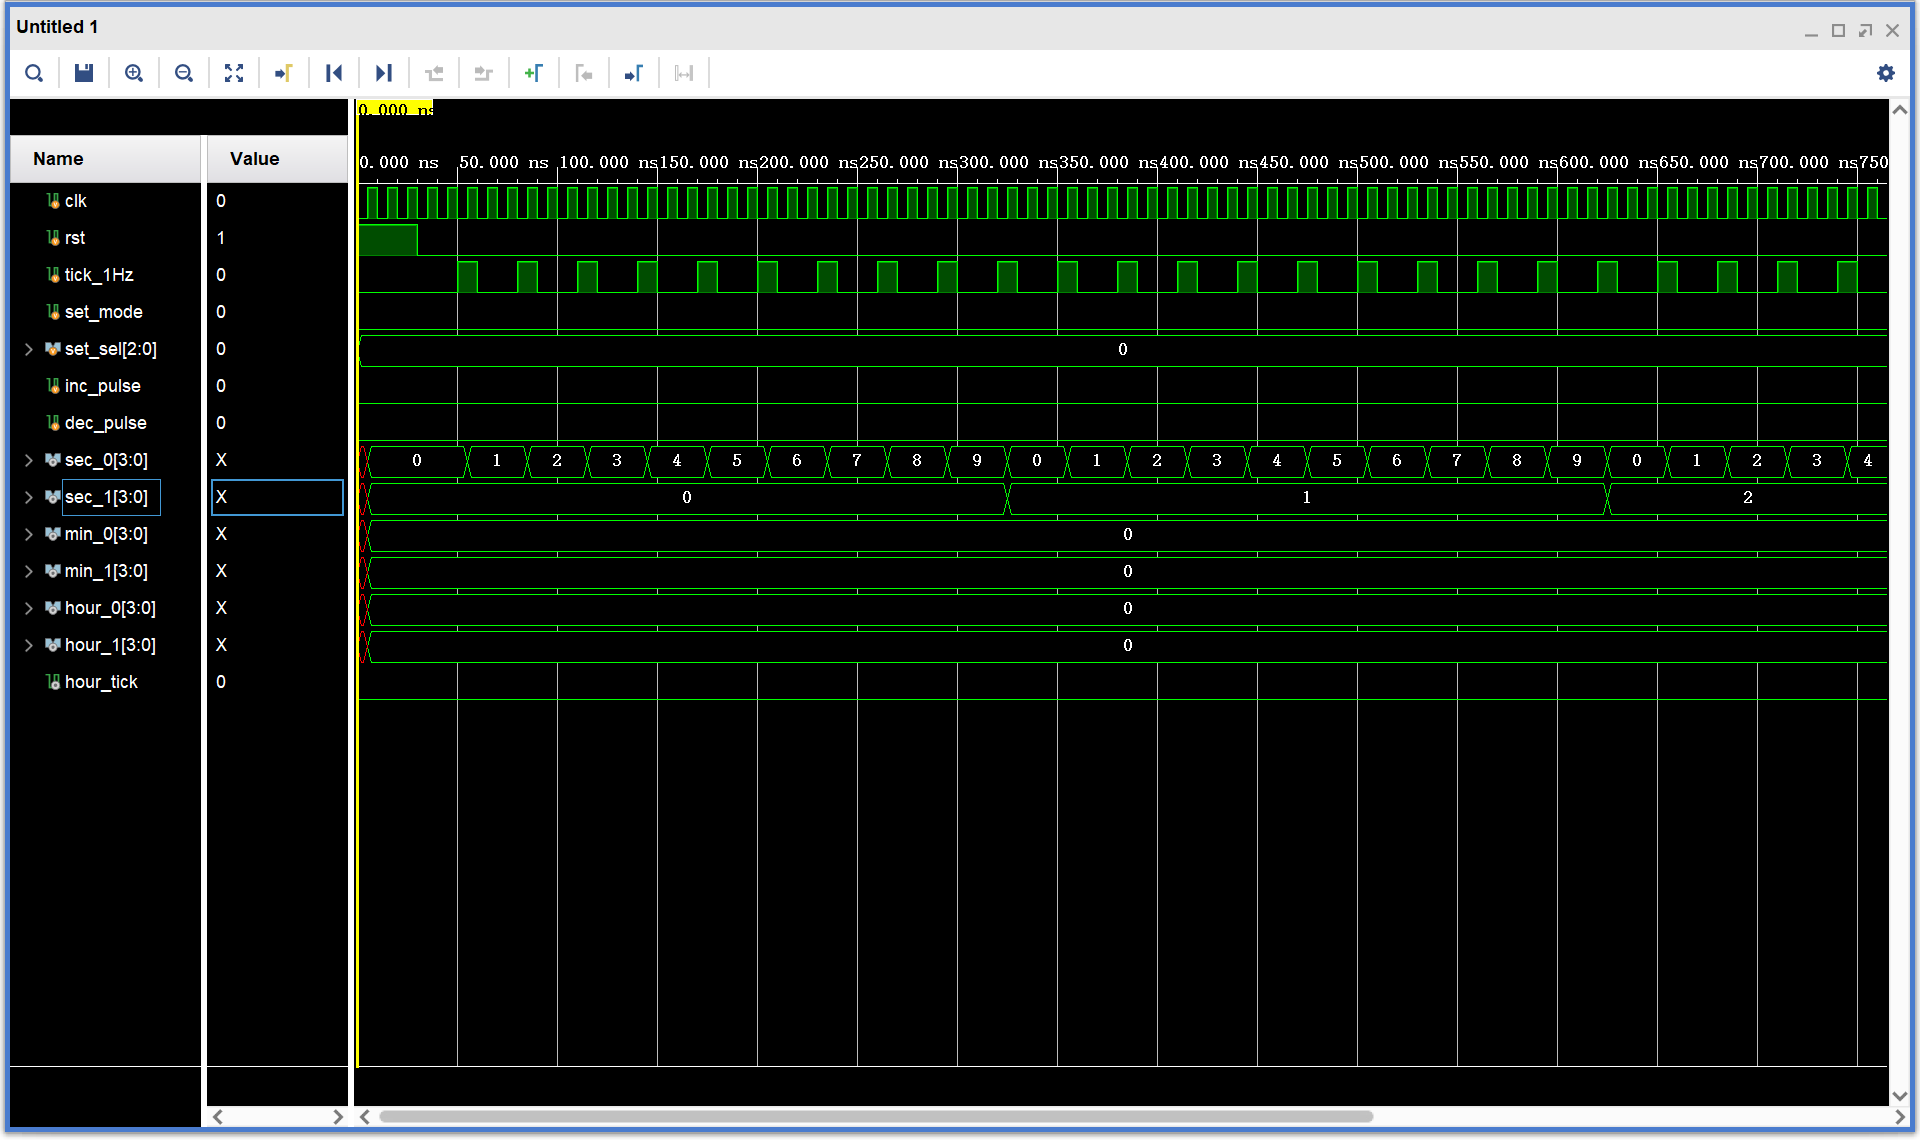
\includegraphics[width=\linewidth]{sim/仿真图片/Sim_time_counter.png}
        \caption{计时进位仿真波形}
    \end{minipage}
    \hfill
    \begin{minipage}{0.48\textwidth}
        \centering
        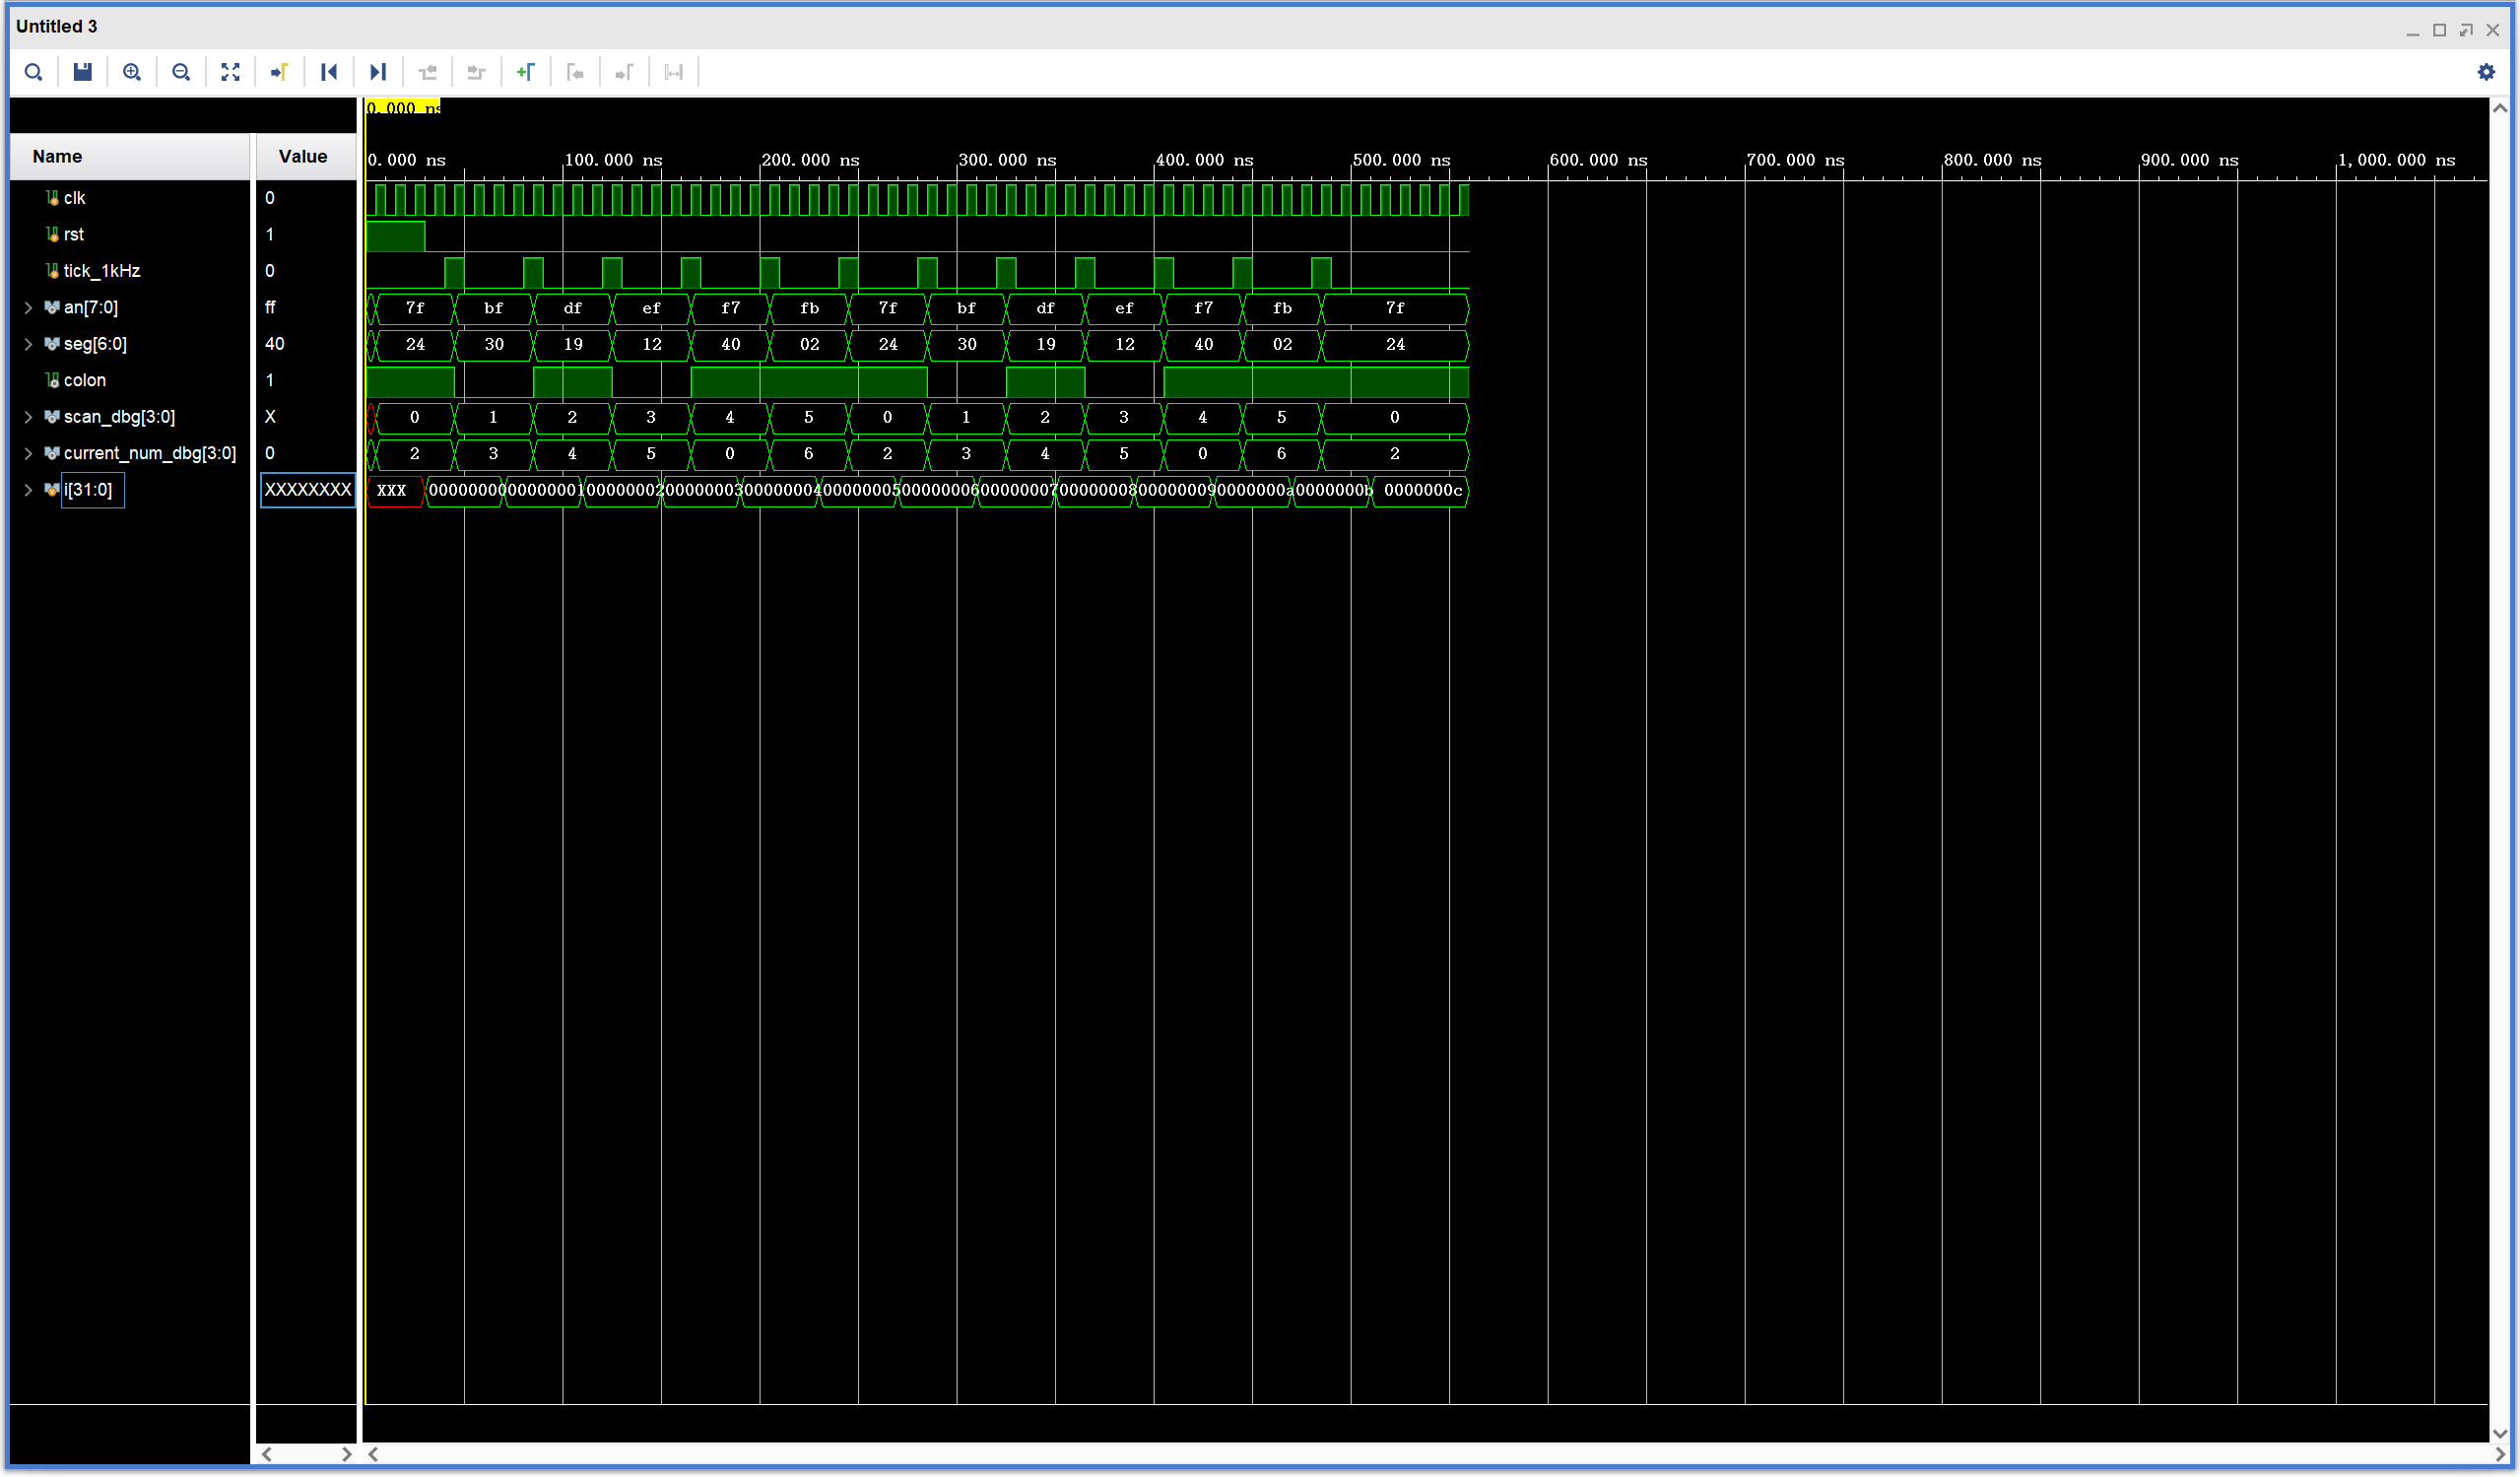
\includegraphics[width=\linewidth]{sim/仿真图片/Sim_digit_display.png}
        \caption{数码管动态扫描仿真波形}
    \end{minipage}
\end{figure}

\begin{figure}[htbp]
    \centering
    \begin{minipage}{0.48\textwidth}
        \centering
        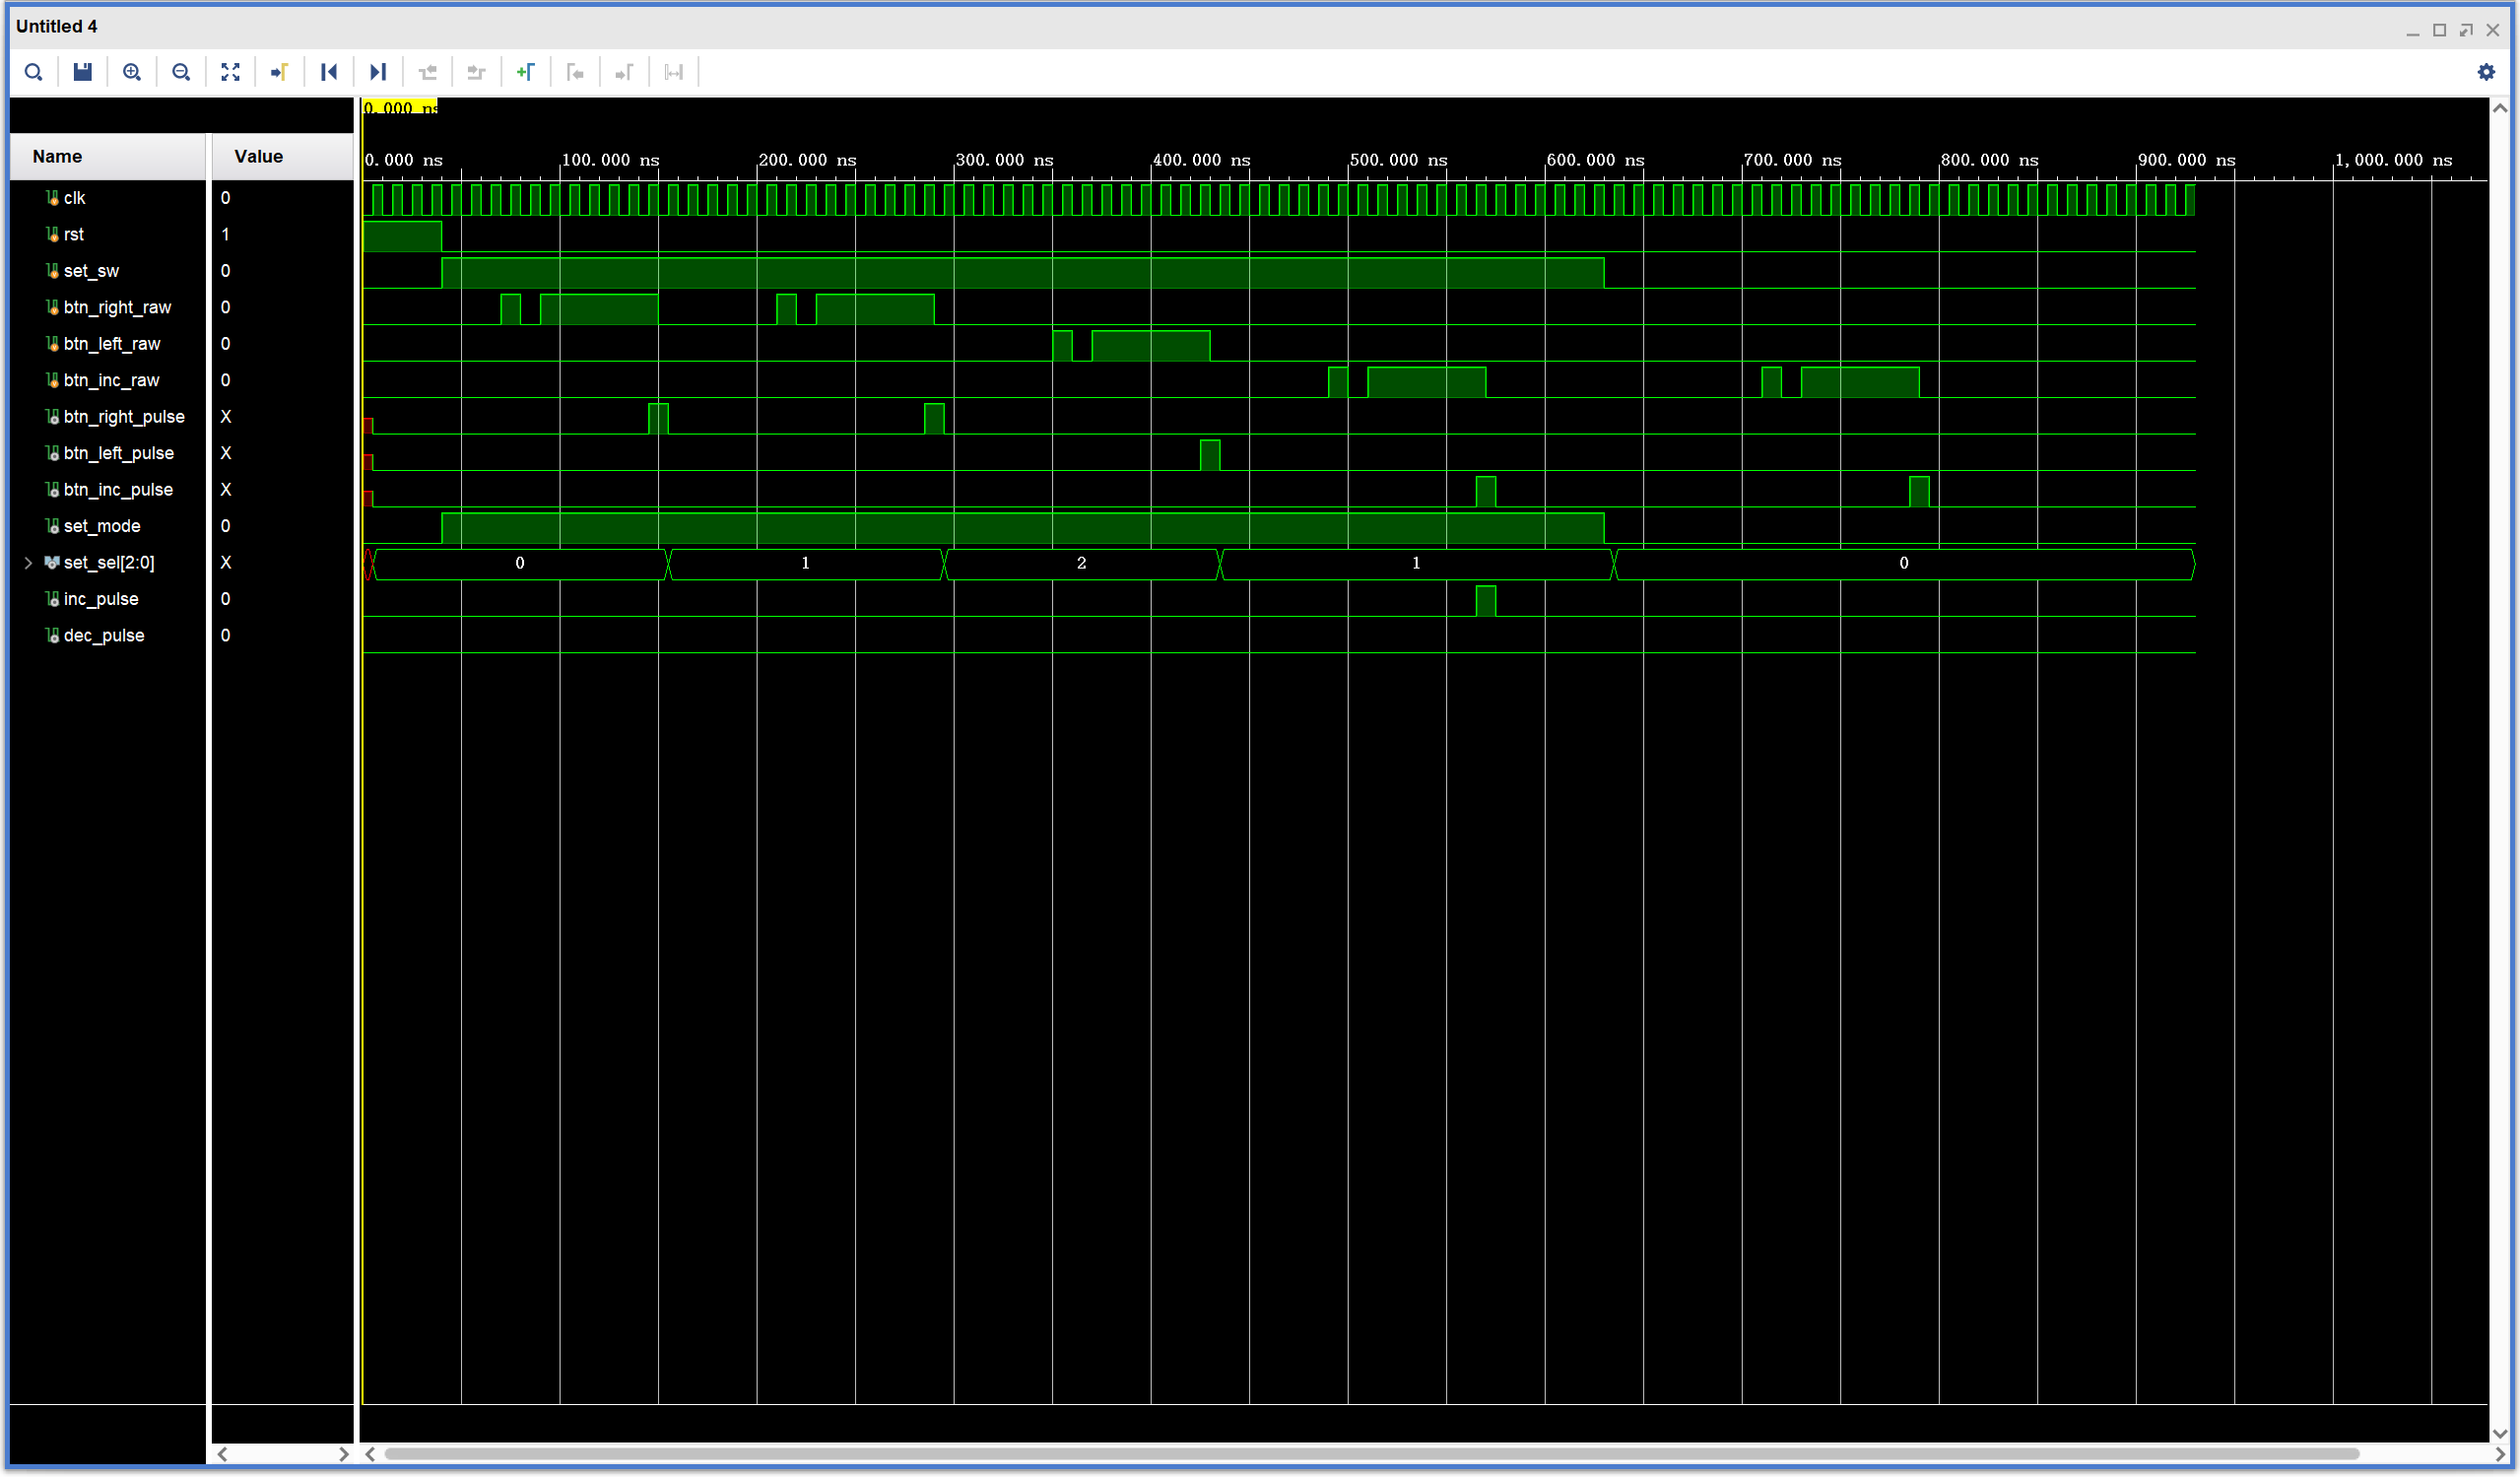
\includegraphics[width=\linewidth]{sim/仿真图片/Sim_set_time_debounce.png}
        \caption{校时与按键消抖仿真波形}
    \end{minipage}
    \hfill
    \begin{minipage}{0.48\textwidth}
        \centering
        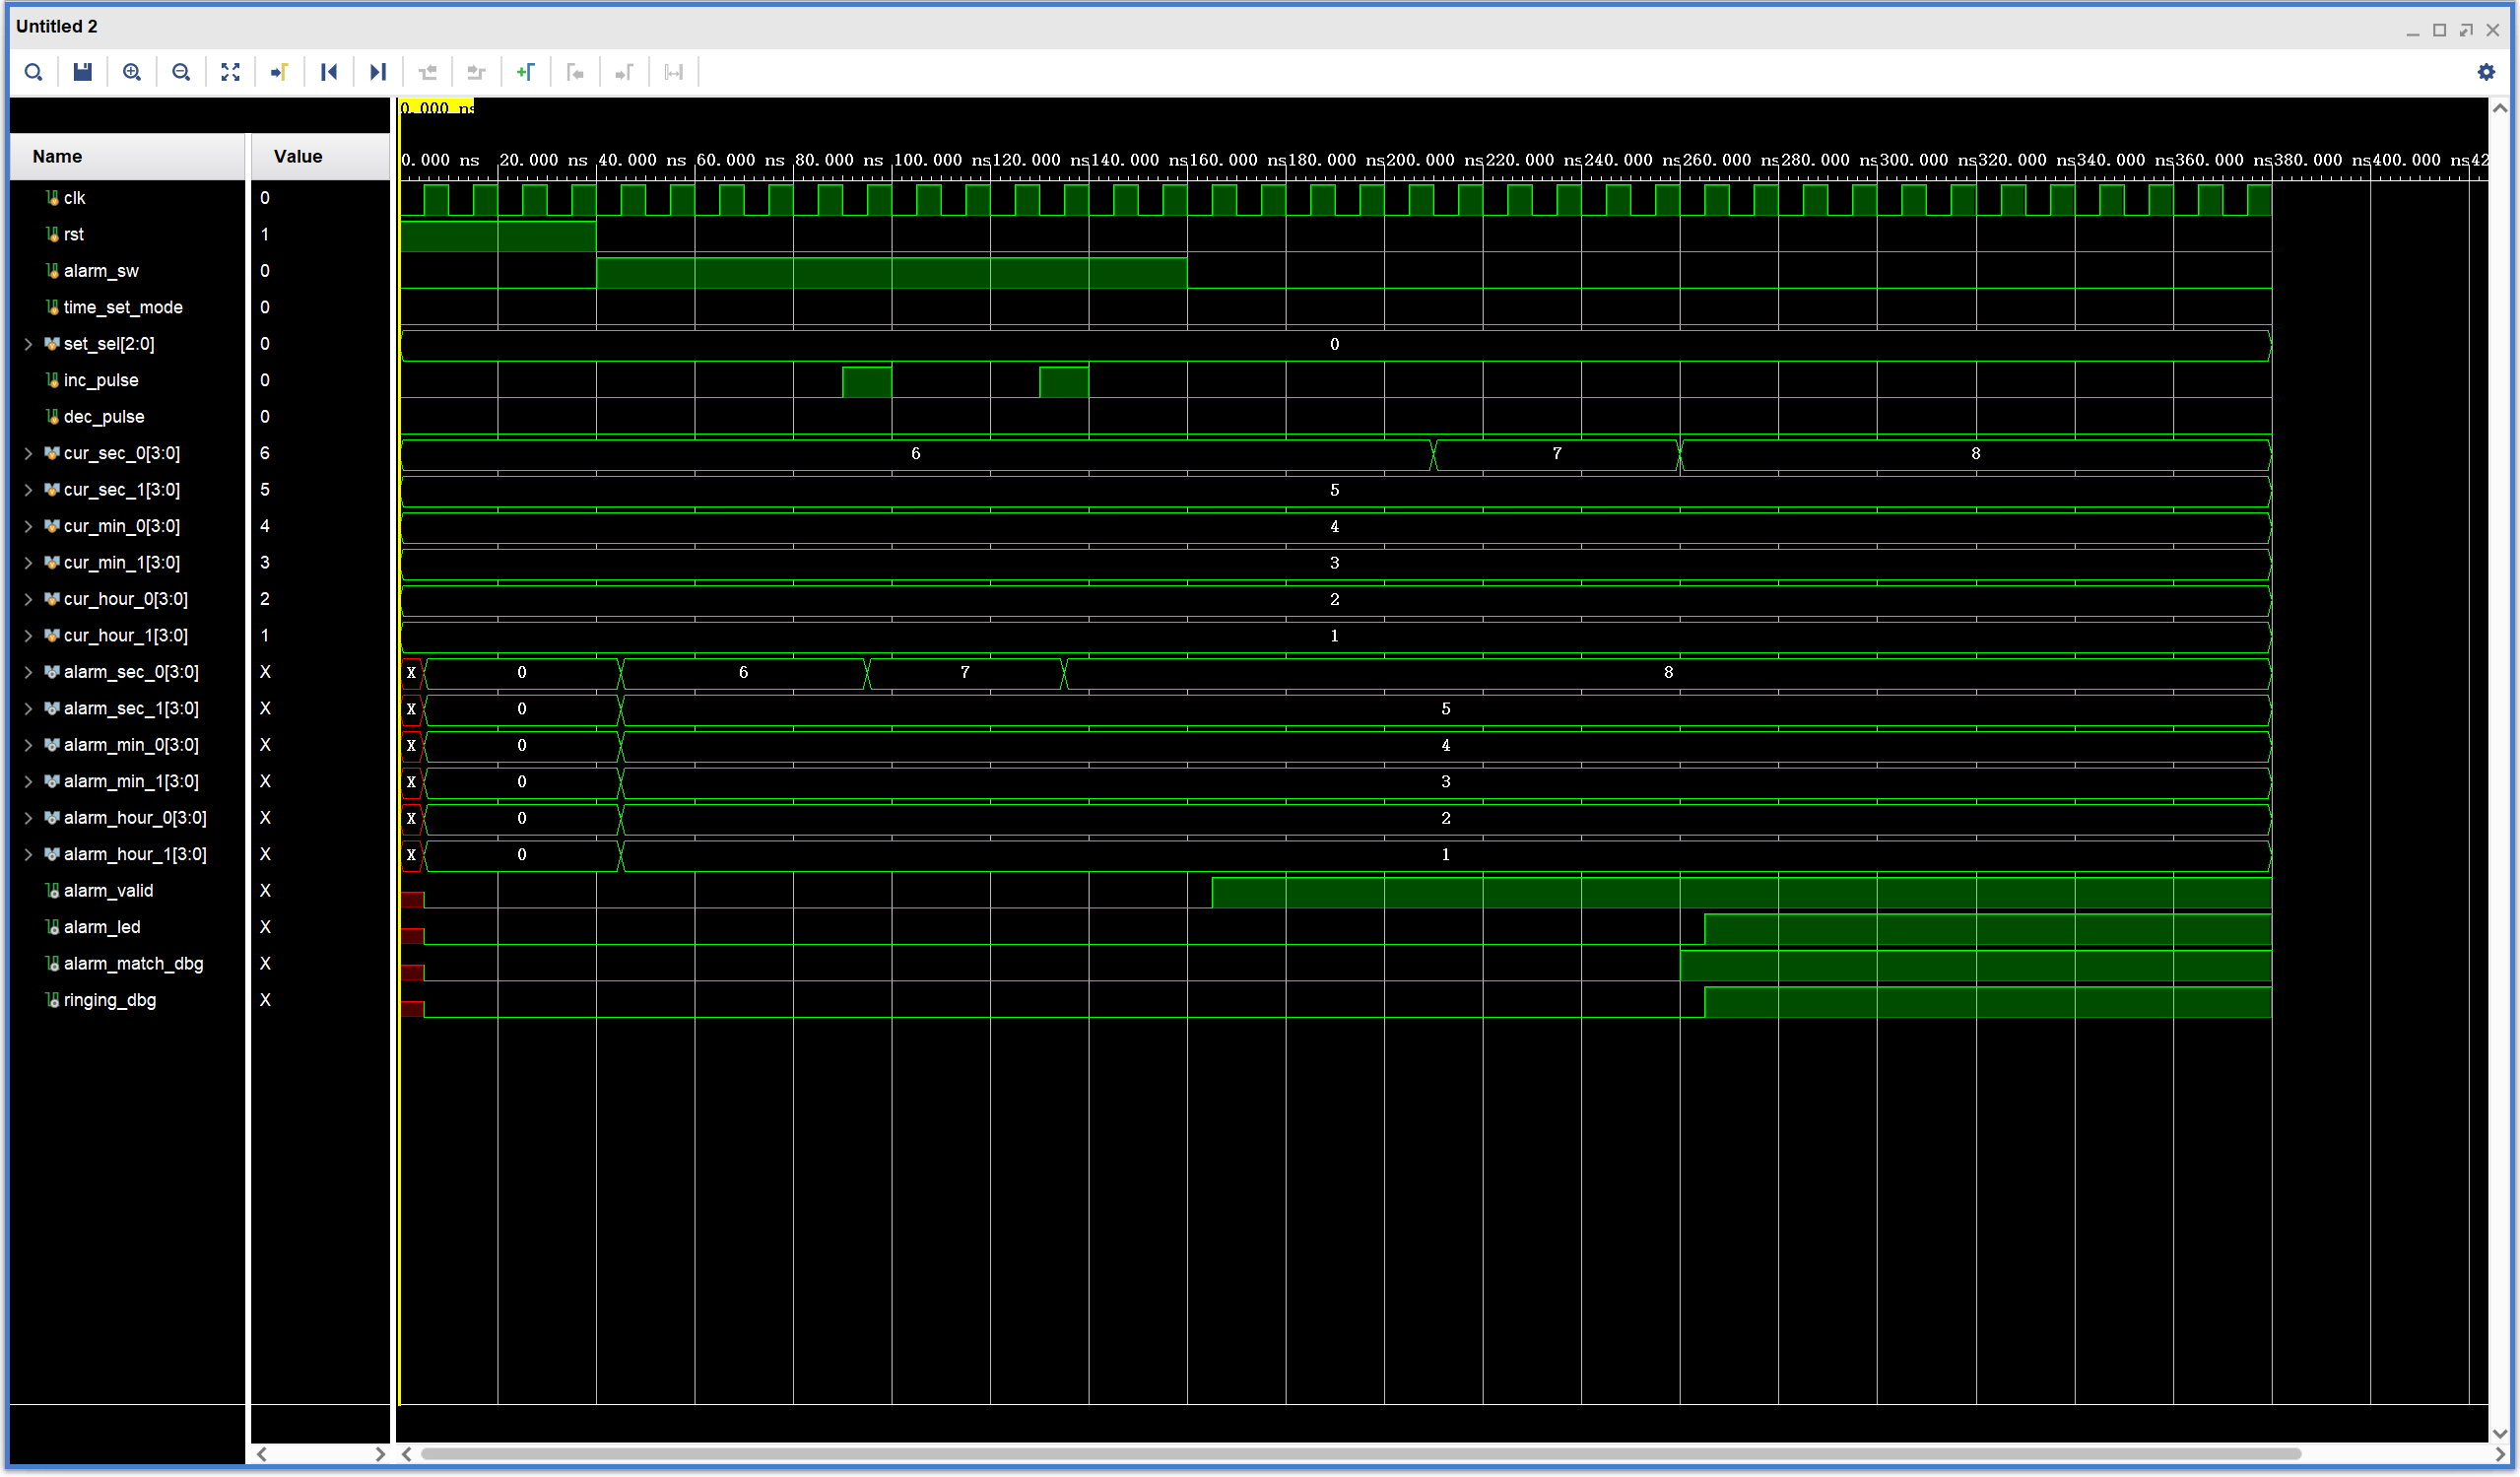
\includegraphics[width=\linewidth]{sim/仿真图片/Sim_alarm.png}
        \caption{闹钟触发仿真波形}
    \end{minipage}
\end{figure}

由图中的计时进位波形可以看到，在每次 \texttt{tick\_1Hz} 有效后，秒个位 \texttt{sec\_0} 依次加一。当 \texttt{sec\_0} 从 9 回到 0 时，秒十位 \texttt{sec\_1} 加一，说明秒个位到秒十位的进位逻辑正确。分钟和小时信号在该段仿真中保持不变，符合当前测试只验证秒计数进位的设置。

数码管扫描仿真中，输入时间被固定为 23:45:06。可以看到 \texttt{scan\_dbg} 按照 0、1、2、3、4、5 的顺序循环变化，对应的 \texttt{current\_num\_dbg} 依次为 2、3、4、5、0、6，正好对应 23:45:06 六位数字。同时，位选信号 \texttt{an} 依次变化，说明数码管能够按照动态扫描的方式逐位显示。

校时与按键消抖仿真中，原始按键信号 \texttt{btn\_right\_raw}、\texttt{btn\_left\_raw} 和 \texttt{btn\_inc\_raw} 在按下时存在短时间跳变，但经过消抖模块后，\texttt{btn\_right\_pulse}、\texttt{btn\_left\_pulse} 和 \texttt{btn\_inc\_pulse} 只产生单个短脉冲。进入校时模式后，右键使 \texttt{set\_sel} 从 0 变为 1，再变为 2，左键又使其回到 1，说明校时位选择逻辑正确；退出校时模式后 \texttt{set\_sel} 回到 0。

闹钟仿真中，当前时间初始设置为 12:34:56。进入闹钟设置模式后，闹钟时间先复制当前时间，随后通过两次加一脉冲将闹钟秒个位从 6 调整到 8。退出闹钟设置后，\texttt{alarm\_valid} 置 1；当当前时间从 12:34:57 变为 12:34:58 时，\texttt{alarm\_match\_dbg} 变为有效，随后 \texttt{ringing\_dbg} 和 \texttt{alarm\_led} 置 1，说明闹钟匹配和报警输出逻辑正确。

\subsection{实验结果及分析}

烧录程序到 FPGA 开发板后，我按照功能点设计了几个测试用例。测试时主要观察六位数码管显示、校时指示灯、闹钟 LED 以及按键响应情况。测试结果如表所示。

\begin{table}[htbp]
    \centering
    \caption{开发板功能测试用例}
    \renewcommand{\arraystretch}{1.2}
    \begin{tabular}{p{0.15\textwidth}p{0.28\textwidth}p{0.28\textwidth}p{0.18\textwidth}}
        \toprule
        测试项目 & 操作方法 & 预期结果 & 实际结果 \\
        \midrule
        复位测试 & 按下复位键 & 数字钟回到 00:00:00，各报警输出关闭 & 与预期一致 \\
        正常计时 & 复位后等待一段时间 & 秒位每秒加一，满 60 秒后分钟加一 & 与预期一致 \\
        校时测试 & 打开校时开关，按左右键选择位，再按加减键修改 & 当前选中位发生变化，未选中位保持不变 & 与预期一致 \\
        按键消抖 & 单次按下加一或减一按键 & 数字只变化一次，不连续跳变 & 与预期一致 \\
        闹钟设置 & 打开闹钟开关，设置目标时间后退出 & 闹钟时间被保存，显示恢复为当前时间 & 与预期一致 \\
        闹钟触发 & 等待当前时间到达闹钟时间 & 闹钟 LED 闪烁一段时间后关闭 & 与预期一致 \\
        整点报时 & 将时间调到接近整点并继续计时 & 分钟从 59 进位到下一小时时产生报时信号 & 与预期一致 \\
        \bottomrule
    \end{tabular}
\end{table}

从测试结果看，数字钟的基本计时功能能够正常工作。复位后显示值回到 00:00:00，正常运行时秒位稳定递增，秒位满 59 后能够正确向分钟进位，说明时分秒级联计数逻辑满足设计要求。

校时功能测试中，进入校时模式后，可以通过左右按键切换当前修改位，再通过加一、减一按键修改数值。按键单次按下时，数值只变化一次，没有出现明显的连续跳变，说明按键消抖和单脉冲处理起到了作用。小时位测试时没有出现 24、29 等非法时间，说明小时计数范围限制正确。

闹钟测试中，打开闹钟设置开关后，数码管显示切换为闹钟时间；设置完成并退出后，系统继续显示当前时间。当当前时间运行到设定的闹钟时间时，闹钟 LED 被点亮并闪烁，持续一段时间后自动关闭。整点报时测试中，当分钟从 59 进位到下一小时时，报时输出能够短暂有效，说明整点检测逻辑正确。

\subsection{测试结果照片}

测试照片主要记录开发板在正常计时、校时、闹钟设置和闹钟触发时的运行状态。照片排版如下。

\begin{figure}[htbp]
    \centering
    \testphoto{figures/test_normal.jpg}{正常计时显示}{请放入 figures/test\_normal.jpg}
    \hfill
    \testphoto{figures/test_set_time.jpg}{校时模式显示}{请放入 figures/test\_set\_time.jpg}
\end{figure}

\begin{figure}[htbp]
    \centering
    \testphoto{figures/test_alarm_set.jpg}{闹钟设置显示}{请放入 figures/test\_alarm\_set.jpg}
    \hfill
    \testphoto{figures/test_alarm_led.jpg}{闹钟触发显示}{请放入 figures/test\_alarm\_led.jpg}
\end{figure}

\subsection{遇到问题及解决办法}

\begin{enumerate}
    \item 数码管显示位序一开始是反的。刚开始只看代码里小时、分钟、秒的顺序，没有仔细对照开发板数码管的位选连接，导致显示出来的数字位置不符合预期。后来逐位测试 \texttt{an} 信号，把小时十位到秒个位的位选顺序重新对应，显示才正常。
    \item 小时会出现 29 这种错误时间。原因是小时不能直接用两个普通十进制计数器实现，否则十位为 2 时个位仍可能数到 9。后来单独写了小时计数逻辑，在小时十位为 2 时限制小时个位最大为 3。
    \item 按键一次触发多次。刚开始直接把按键输入接到校时逻辑，结果按一次数字会跳好几次。后来加入消抖和单脉冲模块，只在按键稳定按下时输出一个脉冲。
    \item 校时模式和正常计时会互相影响。最开始校时时 1 Hz 计时脉冲仍然可能改变当前时间，导致手动调好的数值又被自动计时改掉。解决方法是在进入校时模式后屏蔽普通计时使能，只允许按键脉冲修改当前选中的位。
    \item 闹钟显示和当前时间显示容易混在一起。加入闹钟功能后，需要在设置闹钟时显示闹钟时间，退出后恢复显示当前时间。后来在顶层模块中加入显示数据选择逻辑，用 \texttt{alarm\_sw} 决定送到数码管显示模块的是当前时间还是闹钟时间。
\end{enumerate}

\end{document}
